\documentclass{article}
\usepackage[a4paper,margin=1.5cm]{geometry}
\usepackage{tikz}
\usetikzlibrary{calc,angles,quotes}
\usepackage{fontspec}
\setmainfont{Khmer OS Battambang}
\definecolor{brandNavy}{RGB}{20, 45, 95}
\definecolor{brandCrimson}{RGB}{185, 25, 40}
\definecolor{brandTealBg}{RGB}{238, 246, 248}

\begin{document}
\begin{center}
  % Exercise 12
  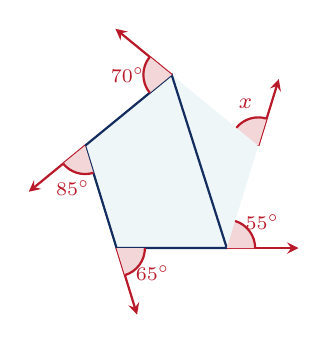
\begin{tikzpicture}[scale=1.0]
    \coordinate (A) at (0, 1.35);
    \coordinate (B) at (-1.1, 0.45);
    \coordinate (C) at (-0.7, -0.85);
    \coordinate (D) at (0.7, -0.85);
    \coordinate (E) at (1.1, 0.45);
    
    \fill[brandTealBg] (A) -- (B) -- (C) -- (D) -- (E) -- cycle;
    \draw[thick, brandNavy] (A) -- (B) -- (C) -- (D) -- cycle;
    
    \coordinate (XA) at ($(E)!1.65!(A)$);
    \coordinate (XB) at ($(A)!1.65!(B)$);
    \coordinate (XC) at ($(B)!1.65!(C)$);
    \coordinate (XD) at ($(C)!1.65!(D)$);
    \coordinate (XE) at ($(D)!1.65!(E)$);
    
    \draw[thick, brandCrimson, ->, >=stealth] (A) -- (XA);
    \draw[thick, brandCrimson, ->, >=stealth] (B) -- (XB);
    \draw[thick, brandCrimson, ->, >=stealth] (C) -- (XC);
    \draw[thick, brandCrimson, ->, >=stealth] (D) -- (XD);
    \draw[thick, brandCrimson, ->, >=stealth] (E) -- (XE);
    
    \pic [draw, brandCrimson, thick, fill=brandCrimson!18, angle radius=0.36cm] {angle = XA--A--B};
    \pic [draw, brandCrimson, thick, fill=brandCrimson!18, angle radius=0.36cm] {angle = XB--B--C};
    \pic [draw, brandCrimson, thick, fill=brandCrimson!18, angle radius=0.36cm] {angle = XC--C--D};
    \pic [draw, brandCrimson, thick, fill=brandCrimson!18, angle radius=0.36cm] {angle = XD--D--E};
    \pic [draw, brandCrimson, thick, fill=brandCrimson!18, angle radius=0.36cm] {angle = XE--E--A};
    
    % Labels exactly inside each exterior angle opening
    \node[font=\fontsize{7.5}{7.5}\selectfont\bfseries, color=brandCrimson] at ($(A)+(180:0.56cm)$) {$70^\circ$};
    \node[font=\fontsize{7.5}{7.5}\selectfont\bfseries, color=brandCrimson] at ($(B)+(254:0.56cm)$) {$85^\circ$};
    \node[font=\fontsize{7.5}{7.5}\selectfont\bfseries, color=brandCrimson] at ($(C)+(325:0.56cm)$) {$65^\circ$};
    \node[font=\fontsize{7.5}{7.5}\selectfont\bfseries, color=brandCrimson] at ($(D)+(36:0.56cm)$) {$55^\circ$};
    \node[font=\fontsize{8.5}{8.5}\selectfont\bfseries, color=brandCrimson] at ($(E)+(107:0.56cm)$) {$x$};
  \end{tikzpicture}
  \hspace{2cm}
  % Exercise 13
  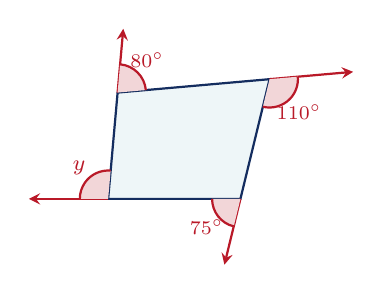
\begin{tikzpicture}[scale=1.0]
    \coordinate (D) at (0, 0);
    \coordinate (A) at (0.12, 1.35);
    \coordinate (B) at (2.05, 1.52);
    \coordinate (C) at (1.68, 0);

    \fill[brandTealBg] (A) -- (B) -- (C) -- (D) -- cycle;
    \draw[thick, brandNavy] (A) -- (B) -- (C) -- (D) -- cycle;

    \coordinate (XA) at ($(D)!1.6!(A)$);
    \coordinate (XB) at ($(A)!1.55!(B)$);
    \coordinate (XC) at ($(B)!1.55!(C)$);
    \coordinate (XD) at ($(C)!1.6!(D)$);

    \draw[thick, brandCrimson, ->, >=stealth] (A) -- (XA);
    \draw[thick, brandCrimson, ->, >=stealth] (B) -- (XB);
    \draw[thick, brandCrimson, ->, >=stealth] (C) -- (XC);
    \draw[thick, brandCrimson, ->, >=stealth] (D) -- (XD);

    \pic [draw, brandCrimson, thick, fill=brandCrimson!18, angle radius=0.36cm] {angle = B--A--XA};
    \pic [draw, brandCrimson, thick, fill=brandCrimson!18, angle radius=0.36cm] {angle = C--B--XB};
    \pic [draw, brandCrimson, thick, fill=brandCrimson!18, angle radius=0.36cm] {angle = D--C--XC};
    \pic [draw, brandCrimson, thick, fill=brandCrimson!18, angle radius=0.36cm] {angle = A--D--XD};

    % Labels exactly inside each exterior angle opening
    \node[font=\fontsize{7.5}{7.5}\selectfont\bfseries, color=brandCrimson] at ($(A)+(48:0.56cm)$) {$80^\circ$};
    \node[font=\fontsize{7.5}{7.5}\selectfont\bfseries, color=brandCrimson] at ($(B)+(-48:0.56cm)$) {$110^\circ$};
    \node[font=\fontsize{7.5}{7.5}\selectfont\bfseries, color=brandCrimson] at ($(C)+(220:0.56cm)$) {$75^\circ$};
    \node[font=\fontsize{8.5}{8.5}\selectfont\bfseries, color=brandCrimson] at ($(D)+(133:0.54cm)$) {$y$};
  \end{tikzpicture}
\end{center}
\end{document}
